

\chapter*{1 Introduction}
\label{intro}
\addcontentsline{toc}{chapter}{1 Introduction}

In order to solve the problem as stated in the \color{blue}introduction\color{black}, a solution that allows \hyperref[listAbr]{ARM}-type processors to be mimicked on standard \hyperref[listAbr]{PC} processors is needed. Since most \hyperref[listAbr]{PC}s make use of either intel\textsuperscript{{\tiny{\textregistered}}} or AMD\textsuperscript{{\tiny{\textregistered}}} \hyperref[listAbr]{CPU}'s (which are x86 based architectures - an ubiquitous iteration of \hyperref[listAbr]{CISC}), emulation or simulation is indeed required. This is because, on a machine level, \hyperref[listAbr]{CISC} architecture is incompatible with \hyperref[listAbr]{RISC} assembly language.
It has been established that \hyperref[listAbr]{RISC} architecture will be mimicked on \hyperref[listAbr]{CISC} machines in order to evaluate student code. The degree of mimicry needed depends largely on the application. Whilst emulation mimics a pertaining architecture relatively closely, simulation does so more loosely. Emulation attempts to duplicate one device as accurately as possible in another environment. Simulation, by contrast, is not concerned with low-level duplication of devices, but instead mimics high-level behaviour.\cite{Chris}
In the following chapters, both emulators and simulators will be evaluated as plausible solutions to the problem: \textbf{How can various student generated C and ARM language assembly code, compiled for RISC architectures, be tested on a single x86 (CISC) architecture PCs?} 

\begin{figure}[H]
\begin{center}
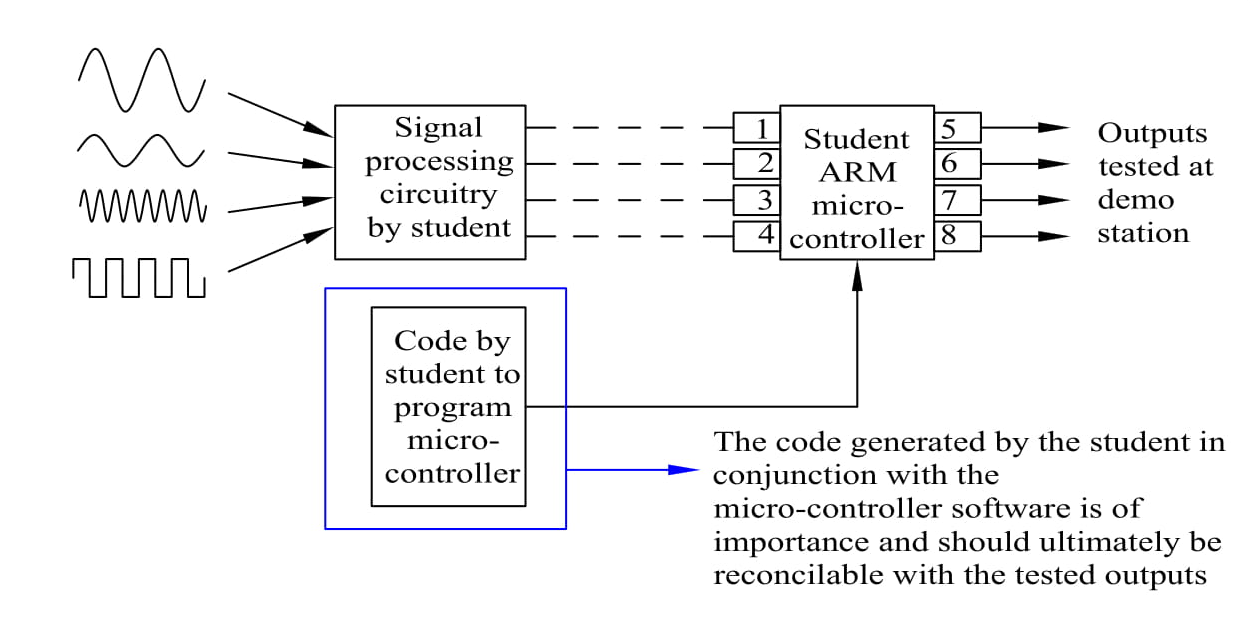
\includegraphics[width = 155mm]{diagram1.png}
\end{center}
\end{figure}
